% Manually authored vector schematic for the CMAME graphical abstract.
% It contains only the audited study design and reported evidence boundaries;
% no generative-AI artwork or reconstructed experimental field is used.
\documentclass{article}
\usepackage[paperwidth=13.833in,paperheight=5.531in,margin=0in]{geometry}
\usepackage{tikz}
\usetikzlibrary{arrows.meta}
\pagestyle{empty}
\begin{document}
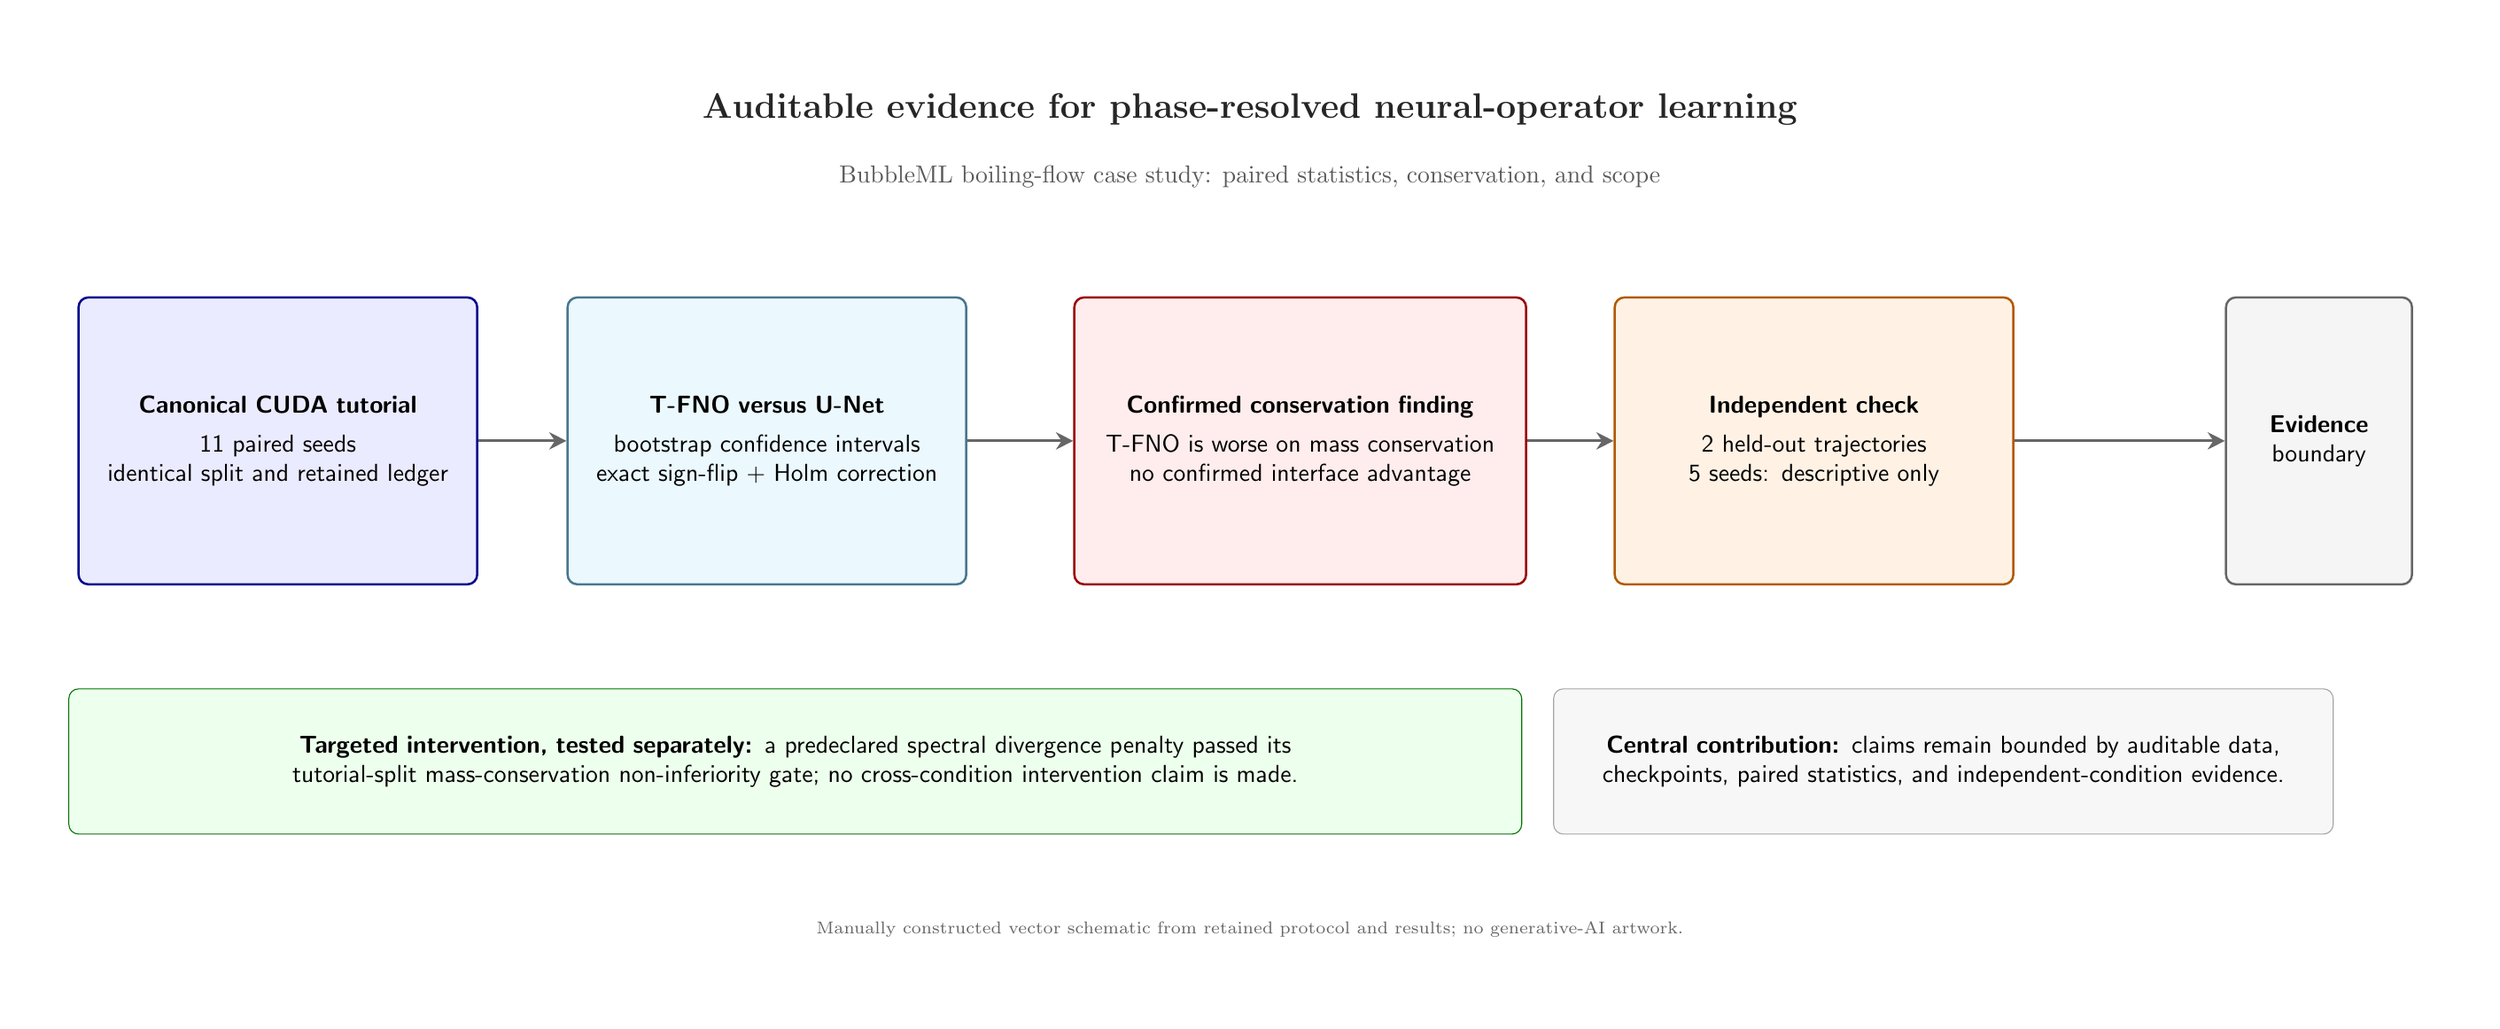
\begin{tikzpicture}[x=1in,y=1in,font=\sffamily]
  \path[use as bounding box] (0,0) rectangle (13.833,5.531);
  \fill[white] (0,0) rectangle (13.833,5.531);
  \node[font=\bfseries\Large,text=black!85] at (6.916,5.05)
    {Auditable evidence for phase-resolved neural-operator learning};
  \node[font=\normalsize,text=black!65] at (6.916,4.67)
    {BubbleML boiling-flow case study: paired statistics, conservation, and scope};

  \tikzset{box/.style n args={3}{draw=#1,line width=.9pt,fill=#2,rounded corners=4pt,
    minimum width=#3,minimum height=1.62in,align=center,text width=#3-0.30in,
    inner sep=7pt}, arrow/.style={-{Stealth[length=7pt,width=7pt]},line width=1.15pt,draw=black!60}}

  \node[box={blue!55!black}{blue!8}{2.25in}] (cuda) at (1.43,3.18)
    {\textbf{Canonical CUDA tutorial}\\[4pt]
     11 paired seeds\\
     identical split and retained ledger};
  \node[box={cyan!50!black}{cyan!8}{2.25in}] (compare) at (4.19,3.18)
    {\textbf{T-FNO versus U-Net}\\[4pt]
     bootstrap confidence intervals\\
     exact sign-flip + Holm correction};
  \node[box={red!60!black}{red!7}{2.55in}] (finding) at (7.20,3.18)
    {\textbf{Confirmed conservation finding}\\[4pt]
     T-FNO is worse on mass conservation\\
     no confirmed interface advantage};
  \node[box={orange!70!black}{orange!10}{2.25in}] (check) at (10.10,3.18)
    {\textbf{Independent check}\\[4pt]
     2 held-out trajectories\\
     5 seeds: descriptive only};
  \node[box={black!60}{black!4}{1.05in}] (boundary) at (12.95,3.18)
    {\textbf{Evidence}\\
     boundary};

  \draw[arrow] (cuda.east) -- (compare.west);
  \draw[arrow] (compare.east) -- (finding.west);
  \draw[arrow] (finding.east) -- (check.west);
  \draw[arrow] (check.east) -- (boundary.west);

  \node[draw=green!45!black,fill=green!7,rounded corners=4pt,minimum width=8.20in,
    minimum height=.82in,align=center,text width=7.85in,inner sep=6pt] at (4.35,1.37)
    {\textbf{Targeted intervention, tested separately:} a predeclared spectral divergence penalty
    passed its tutorial-split mass-conservation non-inferiority gate; no cross-condition intervention claim is made.};
  \node[draw=black!35,fill=black!3,rounded corners=4pt,minimum width=4.40in,
    minimum height=.82in,align=center,text width=4.05in,inner sep=6pt] at (10.83,1.37)
    {\textbf{Central contribution:} claims remain bounded by auditable data, checkpoints,
    paired statistics, and independent-condition evidence.};
  \node[font=\scriptsize,text=black!60] at (6.916,.42)
    {Manually constructed vector schematic from retained protocol and results; no generative-AI artwork.};
\end{tikzpicture}
\end{document}
